\bta{2019}

\section{Use of English}

\noindent
\textbf{Directions:}\\
Read the following text. Choose the best word(s) for each
numbered blank and mark A, B, C or D on the ANSWER SHEET. (10 points)



\TiGanSpace

Today we live in a world where GPS systems, digital maps, and
other navigation apps are available on our smartphones. \cloze of us just
walk straight into the woods without a phone. But phones  \cloze  on batteries,
and batteries can die faster than we realize.  \cloze  you get lost without a
phone or a compass, and you  \cloze  can't find north, we have a few tricks to
help you navigate  \cloze  to civilization, one of which is to follow the land.


When you find yourself  \cloze  a trail, but not in a completely  \cloze  area of land,
you have to answer two questions: Which  \cloze  is downhill, in this
particular area? And where is the nearest water source? Humans
overwhelmingly live in valleys, and on supplies of fresh water.  \cloze , if
you head downhill, and follow any H\textsubscript{2}O you find, you should  \cloze  see signs
of people. 

If you've explored the area before, keep an eye out for
familiar sights---you may be  \cloze  how quickly identifying a distinctive
rock or tree can restore your bearings.

 Another  \cloze  : Climb high
and look for signs of human habitation.  \cloze  , even in dense forest, you
should be able to  \cloze  gaps in the tree line due to roads, train tracks,
and other paths people carve  \cloze  the woods. Head toward these  \cloze  to find
a way out. At night, scan the horizon for  \cloze  light sources, such as
fires and streetlights, then walk toward the glow of light pollution.

 \cloze  , assuming you're lost in an area humans tend to frequent,
look for the  \cloze  we leave on the landscape. Trail blazes, tire tracks,
and other features can  \cloze  you to civilization.

\newpage

\begin{enumerate}
	%\renewcommand{\labelenumi}{\arabic{enumi}.}
	% A(\Alph) a(\alph) I(\Roman) i(\roman) 1(\arabic)
	%设定全局标号series=example	%引用全局变量resume=example
	%[topsep=-0.3em,parsep=-0.3em,itemsep=-0.3em,partopsep=-0.3em]
	%可使用leftmargin调整列表环境左边的空白长度 [leftmargin=0em]
	\item
\fourchoices
{Some}
{Most}
{Few}
{All}



\item

\fourchoices
{put}
{take}
{run}
{come}



\item

\fourchoices
{Since}
{If}
{Though}
{Until}




\item

\fourchoices
{formally}
{relatively}
{gradually}
{literally}



\item

\fourchoices
{back}
{next}
{around}
{away}



\item

\fourchoices
{onto}
{off}
{across}
{along}



\item

\fourchoices
{unattractive}
{uncrowded}
{unchanged}
{unfamiliar}


\item

\fourchoices
{site}
{point}
{way}
{place}



\item

\fourchoices
{So}
{Yet}
{Instead}
{Besides}




\item

\fourchoices
{immediately}
{intentionally}
{unexpectedly}
{eventually}




\item

\fourchoices
{surprised}
{annoyed}
{frightened}
{confused}



\item

\fourchoices
{problem}
{option}
{view}
{result}



\item

\fourchoices
{Above all}
{In contrast}
{On average}
{For example}



\item

\fourchoices
{bridge}
{avoid}
{spot}
{separate}



\item

\fourchoices
{from}
{through}
{beyond}
{under}


\item

\fourchoices
{posts}
{links}
{shades}
{breaks}


\item
\fourchoices
{artificial}
{mysterious}
{hidden}
{limited}


\item
\fourchoices
{Finally}
{Consequently}
{Incidentally}
{Generally}


\item

\fourchoices
{memories}
{marks}
{notes}
{belongings}


\item

\fourchoices
{restrict}
{adapt}
{lead}
{expose}

\end{enumerate}


\vfil

\section{Reading Comprehension}

\noindent
\textbf{Part A}\\
\textbf{Directions:}\\
 Read the following four texts. Answer the questions
after each text by choosing A, B, C or
D. Mark your answers on the
ANSWER SHEET. (40 points)

\newpage

\subsection{Text 1}

Financial regulators in Britain have imposed a rather unusual rule
on the bosses of big banks. Starting next year, any guaranteed bonus of
top executives could be delayed 10 years if their banks are under
investigation for wrongdoing. The main purpose of this ``clawback'' rule
is to hold bankers accountable for harmful risk-taking and to restore
public trust in financial institutions. Yet officials also hope for a
much larger benefit: more long-term decision-making, not only by banks
but by all corporations, to build a stronger economy for future
generations. 

``Short-termism,'' or the desire for quick profits,
has worsened in publicly traded companies, says the Bank of England's
top economist, Andrew Haldane. He quotes a giant of classical economics,
Alfred Marshall, in describing this financial impatience as acting like
``children who pick the plums out of their pudding to eat them at once''
rather than putting them aside to be eaten last. 



The average time
for holding a stock in both the United States and Britain, he notes, has
dropped from seven years to seven months in recent decades. Transient
investors, who demand high quarterly profits from companies, can hinder
a firm's efforts to invest in long-term research or to build up customer
loyalty. This has been dubbed ``quarterly capitalism.'' 


In addition, new digital technologies have allowed more rapid trading of
equities, quicker use of information, and thus shorter attention spans
in financial markets. ``There seems to be a predominance of short-term
thinking at the expense of long-term investing,'' said Commissioner
Daniel Gallagher of the US Securities and Exchange Commission in a
speech this week. 


In the US, \emph{the Sarbanes-Oxley Act of 2002} has
pushed most public companies to defer performance bonuses for senior
executives by about a year, slightly helping reduce ``short-termism.''
In its latest survey of CEO pay, \emph{The Wall Street Journal} finds that ``a
substantial part'' of executive pay is now tied to performance.




Much more could be done to encourage ``long-termism,'' such as
changes in the tax code and quicker disclosure of stock acquisitions. In
France, shareholders who hold onto a company investment for at least two
years can sometimes earn more voting rights in a company. 


Within companies, the right compensation design can provide incentives for
executives to think beyond their own time at the company and on behalf
of all stakeholders. Britain's new rule is a reminder to bankers that
society has an interest in their performance, not just for the short
term but for the long term.

\begin{enumerate}[resume]
	%\renewcommand{\labelenumi}{\arabic{enumi}.}
	% A(\Alph) a(\alph) I(\Roman) i(\roman) 1(\arabic)
	%设定全局标号series=example	%引用全局变量resume=example
	%[topsep=-0.3em,parsep=-0.3em,itemsep=-0.3em,partopsep=-0.3em]
	%可使用leftmargin调整列表环境左边的空白长度 [leftmargin=0em]
	\item
According to Paragraph 1, one motive in imposing the new rule is to \lineread.

\fourchoices
{enhance bankers' sense of responsibility}
{help corporations achieve larger profits}
{build a new system of financial regulation}
{guarantee the bonuses of top executives}


\item
Alfred Marshall is quoted to indicate \lineread.

\fourchoices
{the conditions for generating quick profits}
{governments' impatience in decision-making}
{the solid structure of publicly traded companies}
{``short-termism'' in economic activities}


\item
 It is argued that the influence of transient investment on public
companies can be \lineread.


\fourchoices
{indirect}
{adverse}
{minimal}
{temporary}



\item
The US and France examples are used to illustrate \lineread.


\fourchoices
{the obstacles to preventing ``short-termism''}
{the significance of long-term thinking}
{the approaches to promoting ``long-termism''}
{the prevalence of short-term thinking}


\item
Which of the following would be the best title for the text?

\fourchoices
{Failure of Quarterly Capitalism}
{Patience as a Corporate Virtue}
{Decisiveness Required of Top Executives}
{Frustration of Risk-taking Bankers}


\end{enumerate}



\newpage


\subsection{Text 2}

Grade inflation---the gradual increase in average GPAs
(grade-point averages) over the past few decades---is often considered
a product of a consumer era in higher education, in which students are
treated like customers to be pleased. But another, related force---a
policy often buried deep in course catalogs called ``grade forgiveness''---is helping raise GPAs. 


Grade forgiveness allows students to
retake a course in which they received a low grade, and the most recent
grade or the highest grade is the only one that counts in calculating a
student's overall GPA. 



The use of this little-known practice has
accelerated in recent years, as colleges continue to do their utmost to
keep students in school (and paying tuition) and improve their
graduation rates. When this practice first started decades ago, it was
usually limited to freshmen, to give them a second chance to take a
class in their first year if they struggled in their transition to
college-level courses. But now most colleges, save for many selective
campuses, allow all undergraduates, and even graduate students, to get
their low grades forgiven. 


College officials tend to emphasize
that the goal of grade forgiveness is less about the grade itself and
more about encouraging students to retake courses critical to their
degree program and graduation without incurring a big penalty.
``Ultimately,'' said Jack Miner, Ohio State University's registrar, ``we
see students achieve more success because they retake a course and do
better in subsequent courses or master the content that allows them to
graduate on time.'' 



That said, there is a way in which grade
forgiveness satisfies colleges' own needs as well. For public
institutions, state funds are sometimes tied partly to their success on
metrics such as graduation rates and student retention---so better
grades can, by boosting figures like those, mean more money. And
anything that raises GPAs will likely make students -- who, at the end
of the day, are paying the bill---feel they've gotten a better value
for their tuition dollars, which is another big concern for colleges.



Indeed, grade forgiveness is just another way that universities
are responding to consumers' expectations for higher education. Since
students and parents expect a college degree to lead to a job, it is in
the best interest of a school to turn out graduates who are as qualified
as possible---or at least appear to be. On this, students' and
colleges' incentives seem  \uline{to be aligned}.


\begin{enumerate}[resume]
	%\renewcommand{\labelenumi}{\arabic{enumi}.}
	% A(\Alph) a(\alph) I(\Roman) i(\roman) 1(\arabic)
	%设定全局标号series=example	%引用全局变量resume=example
	%[topsep=-0.3em,parsep=-0.3em,itemsep=-0.3em,partopsep=-0.3em]
	%可使用leftmargin调整列表环境左边的空白长度 [leftmargin=0em]
	\item
 What is commonly regarded as the cause of grade inflation?
\fourchoices
{The change of course catalogs.}
{Students' indifference to GPAs.}
{Colleges' neglect of GPAs.}
{The influence of consumer culture.}



\item
What was the original purpose of grade forgiveness?
\fourchoices
{To help freshmen adapt to college learning.}
{To maintain colleges' graduation rates.}
{To prepare graduates for a challenging future.}
{To increase universities' income from tuition.}


\item
 According to Paragraph 5, grade forgiveness enables colleges to \lineread.

\fourchoices
{obtain more financial support}
{boost their student enrollments}
{improve their teaching quality}
{meet local governments' needs}



\item
What does the phrase ``to be aligned'' (Line 5, Para. 6) most
probably mean?


\fourchoices
{To counterbalance each other.}
{To complement each other.}
{To be identical with each other.}
{To be contradictory to each other.}



\item
The author examines the practice of grade forgiveness by \lineread.

\fourchoices
{assessing its feasibility}
{analyzing the causes behind it}
{comparing different views on it}
{listing its long-run effects}

\end{enumerate}

\newpage

\subsection{Text 3}

This year marks exactly two centuries since the publication of
\emph{Frankenstein; or, The Modern Prometheus}, by Mary Shelley. Even
before the invention of the electric light bulb, the author produced a
remarkable work of speculative fiction that would foreshadow many
ethical questions to be raised by technologies yet to come. 


Today the rapid growth of artificial intelligence (AI) raises fundamental
questions: ``What is intelligence, identity, or consciousness? What
makes humans humans?'' 


What is being called artificial general
intelligence, machines that would imitate the way humans think,
continues to evade scientists. Yet humans remain fascinated by the idea
of robots that would look, move, and respond like humans, similar to
those recently depicted on popular sci-fi TV series such as
``Westworld'' and ``Humans''. 



Just how people think is still far too
complex to be understood, let alone reproduced, says David Eagleman, a
Stanford University neuroscientist. ``We are just in a situation where
there are no good theories explaining what consciousness actually is and
how you could ever build a machine to get there.'' 


But that doesn't
mean crucial ethical issues involving AI aren't at hand. The coming use
of autonomous vehicles, for example, poses thorny ethical questions.
Human drivers sometimes must make split-second decisions. Their
reactions may be a complex combination of instant reflexes, input from
past driving experiences, and what their eyes and ears tell them in that
moment. AI ``vision'' today is not nearly as sophisticated as that of
humans. And to anticipate every imaginable driving situation is a
difficult programming problem. 


Whenever decisions are based on
masses of data, ``you quickly get into a lot of ethical questions,''
notes Tan Kiat How, chief executive of a Singapore-based agency that is
helping the government develop a voluntary code for the ethical use of
AI. Along with Singapore, other governments and mega-corporations are
beginning to establish their own guidelines. Britain is setting up a
data ethics center. India released its AI ethics strategy this spring.



On June 7 Google pledged not to ``design or deploy AI'' that would
cause ``overall harm,'' or to develop AI-directed weapons or use AI for
surveillance that would violate international norms. It also pledged not
to deploy AI whose use would violate international laws or human rights.



While the statement is vague, it represents one starting point. So
does the idea that decisions made by AI systems should be explainable,
transparent, and fair. 


To put it another way: How can we make sure
that the thinking of intelligent machines reflects humanity's highest
values? Only then will they be useful servants and not Frankenstein's
out-of-control monster.


\begin{enumerate}[resume]
	%\renewcommand{\labelenumi}{\arabic{enumi}.}
	% A(\Alph) a(\alph) I(\Roman) i(\roman) 1(\arabic)
	%设定全局标号series=example	%引用全局变量resume=example
	%[topsep=-0.3em,parsep=-0.3em,itemsep=-0.3em,partopsep=-0.3em]
	%可使用leftmargin调整列表环境左边的空白长度 [leftmargin=0em]
	\item
Mary Shelley's novel \emph{Frankenstein} is mentioned because it \lineread.

\fourchoices
{fascinates AI scientists all over the world}
{has remained popular for as long as 200 years}
{involves some concerns raised by AI today}
{has sparked serious ethical controversies}



\item
In David Eagleman's opinion, our current knowledge of consciousness \lineread.

\fourchoices
{helps explain artificial intelligence}
{can be misleading to robot making}
{inspires popular sci-fi TV series}
{is too limited for us to reproduce it}


\item
The solution to the ethical issues brought by autonomous vehicles \lineread.

\fourchoices
{can hardly ever be found}
{is still beyond our capacity}
{causes little public concern}
{has aroused much curiosity}


\item
The author's attitude toward Google's pledges is one of \lineread.


\fourchoices
{affirmation}
{skepticism}
{contempt}
{respect}




\item
Which of the following would be the best title for the text?

\fourchoices
{AI's Future: In the Hands of Tech Giants}
{\emph{Frankenstein}, the Novel Predicting the Age of AI}
{The Conscience of AI: Complex But Inevitable}
{AI Shall Be Killers Once Out of Control}

\end{enumerate}


\newpage

\subsection{Text 4}





States will be able to force more people to pay sales tax when
they make online purchases under a Supreme Court decision Thursday that
will leave shoppers with lighter wallets but is a big financial win for
states. 


The Supreme Court's opinion Thursday overruled a pair of
decades-old decisions that states said cost them billions of dollars in
lost revenue annually. The decisions made it more difficult for states
to collect sales tax on certain online purchases. 


The cases the
court overturned said that if a business was shipping a customer's
purchase to a state where the business didn't have a physical presence
such as a warehouse or office, the business didn't have to collect sales
tax for the state. Customers were generally responsible for paying the
sales tax to the state themselves if they weren't charged it, but most
didn't realize they owed it and few paid. 


Justice Anthony Kennedy
wrote that the previous decisions were flawed. ``Each year the physical
presence rule becomes further removed from economic reality and results
in significant revenue losses to the States,'' he wrote in an opinion
joined by four other justices. Kennedy wrote that the rule ``limited
states' ability to seek long-term prosperity and has prevented market
participants from competing on an even playing field.'' 


The ruling
is a victory for big chains with a presence in many states, since they
usually collect sales tax on online purchases already. Now, rivals will
be charging sales tax where they hadn't before. Big chains have been
collecting sales tax nationwide because they typically have physical
stores in whatever state a purchase is being shipped to. Amazon.com,
with its network of warehouses, also collects sales tax in every state
that charges it, though third-party sellers who use the site don't have
to. 



Until now, many sellers that have a physical presence in only
a single state or a few states have been able to avoid charging sales
taxes when they ship to addresses outside those states. Sellers that use
eBay and Etsy, which provide platforms for smaller sellers, also haven't
been collecting sales tax nationwide. Under the ruling Thursday, states
can pass laws requiring out-of-state sellers to collect the state's
sales tax from customers and send it to the state.


 Retail trade
groups praised the ruling, saying it levels the playing field for local
and online businesses. The losers, said retail analyst Neil Saunders,
are online-only retailers, especially smaller ones. Those retailers may
face headaches complying with various state sales tax laws. The Small
Business \& Entrepreneurship Council advocacy group said in a statement,
``Small businesses and internet entrepreneurs are not well served at all
by this decision.''

\begin{enumerate}[resume]
	%\renewcommand{\labelenumi}{\arabic{enumi}.}
	% A(\Alph) a(\alph) I(\Roman) i(\roman) 1(\arabic)
	%设定全局标号series=example	%引用全局变量resume=example
	%[topsep=-0.3em,parsep=-0.3em,itemsep=-0.3em,partopsep=-0.3em]
	%可使用leftmargin调整列表环境左边的空白长度 [leftmargin=0em]
	\item
The Supreme Court decision Thursday will \lineread.


\fourchoices
{better businesses' relations with states}
{put most online businesses in a dilemma}
{make more online shoppers pay sales tax}
{force some states to cut sales tax}

\item
It can be learned from paragraphs 2 and 3 that the overruled
decisions \lineread.


\fourchoices
{have led to the dominance of e-commerce}
{have cost consumers a lot over the years}
{were widely criticized by online purchasers}
{were considered unfavorable by states}


\item
According to Justice Anthony Kennedy, the physical presence rule has \lineread.



\fourchoices
{hindered economic development}
{brought prosperity to the country}
{harmed fair market competition}
{boosted growth in states' revenue}



\item
Who are most likely to welcome the Supreme Court ruling?

\fourchoices
{Internet entrepreneurs.}
{Big-chain owners.}
{Third-party sellers.}
{Small retailers.}



\item
In dealing with the Supreme Court decision Thursday, the author \lineread.

\fourchoices
{gives a factual account of it and discusses its consequences}
{describes the long and complicated process of its making}
{presents its main points with conflicting views on them}
{cites some cases related to it and analyzes their implications}

\end{enumerate}



\newpage

\noindent
\textbf{Part B}\\
\textbf{Directions:}\\
 The following paragraphs are given in a wrong order.
For Questions 41-45, you are required to reorganize these paragraphs
into a coherent text by choosing from the list A-G and filling them into
the numbered boxes. Paragraphs C and F have been correctly placed. Mark
your answers on the ANSWER SHEET. (10 points)


\begin{listmatch}
\item 
These tools can help you win every argument---not in the
unhelpful sense of beating your opponents but in the better sense of
learning about the issues that divide people. Learning why they disagree
with us and learning to talk and work together with them. If we readjust
our view of arguments---from a verbal fight or tennis game to a
reasoned exchange through which we all gain mutual respect, and
understanding---then we change the very nature of what it means to
``win'' an argument.


\item 
 Of course, many discussions are not so successful. Still, we need
to be careful not to accuse opponents of bad arguments too quickly. We
need to learn how to evaluate them properly. A large part of evaluation
is calling out bad arguments, but we also need to admit good arguments
by opponents and to apply the same critical standards to ourselves.
Humility requires you to recognize weakness in your own arguments and
sometimes also to accept reasons on the opposite side.


\item 
None of these will be easy but you can start even if others
refuse to. Next time you state your position, formulate an argument for
what you claim and honestly ask yourself whether your argument is any
good. Next time you talk with someone who takes a stand, ask them to
give you a reason for their view. Spell out their argument fully and
charitably. Assess its strength impartially. Raise objections and listen
carefully to their replies.


\item 
Carnegie would be right if arguments were fights, which is how we
often think of them. Like physical fights, verbal fights can leave both
sides bloodied. Even when you win, you end up no better off. Your
prospects would be almost as dismal if arguments were even just
competitions---like, say, tennis games. Pairs of opponents hit the ball back and forth until one winner emerges from
all who entered. Everybody else loses. This kind of thinking is why so
many people try to avoid arguments, especially about politics and
religion.


\item 
 In his 1936 work \emph{How to Win Friends and Influence People}, Dale
Carnegie wrote: ``There is only one way\ldots to get the best of an
argument---and that is to avoid it.'' This aversion to arguments is
common, but it depends on a mistaken view of arguments that causes
profound problems for our personal and social lives---and in many ways
misses the point of arguing in the first place.


\item 
These views of arguments also undermine reason. If you see a
conversation as a fight or competition, you can win by cheating as long
as you don't get caught. You will be happy to convince people with bad
arguments. You can call their views stupid, or joke about how ignorant
they are. None of these tricks will help you understand them, their
positions or the issues that divide you, but they can help you win---in
one way.


\item 
There is a better way to win arguments. Imagine that you favor
increasing the minimum wage in our state, and I do not. If you yell,
``Yes,'' and I yell, ``No,'' neither of us learns anything. We neither
understand nor respect each other, and we have no basis for compromise
or cooperation. In contrast, suppose you give a reasonable argument:
that full-time workers should not have to live in poverty. Then I
counter with another reasonable argument: that a higher minimum wage
will force businesses to employ fewer people for less time. Now we can
understand each other's positions and recognize our shared values, since
we both care about needy workers.

\end{listmatch}



\[ 
\begin{tabular}{|c|c|}
	\hline
	41. &  \hspace{1.5em} \\
	\hline
\end{tabular}
\rightarrow
\begin{tabular}{|c|c|}
	\hline
	42. &  \hspace{1.5em} \\
	\hline
\end{tabular}
\rightarrow
\begin{tabular}{|c|}
	\hline
	F \\
	\hline
\end{tabular}
\rightarrow
\begin{tabular}{|c|c|}
	\hline
	43. &  \hspace{1.5em} \\
	\hline
\end{tabular}
\rightarrow
\begin{tabular}{|c|c|}
	\hline
	44. &  \hspace{1.5em} \\
	\hline
\end{tabular}
\rightarrow
\begin{tabular}{|c|}
	\hline
	C \\
	\hline
\end{tabular}
\rightarrow
\begin{tabular}{|c|c|}
	\hline
	45. &  \hspace{1.5em} \\
	\hline
\end{tabular}
\]


\phantom{ \linefill \linefill \linefill \linefill \linefill}


\newpage

\noindent
\textbf{Part C}\\
\textbf{Directions:}\\
 Read the following text carefully and then translate
the underlined segments into Chinese. Write your answers on the ANSWER SHEET. (10 points)


\TiGanSpace


It was only after I started to write a weekly column about the
medical journals, and began to read scientific papers from beginning to
end, that I realised just how bad much of the medical literature
frequently was. I came to recognise various signs of a bad paper: the
kind of paper that purports to show that people who eat more than one
kilo of broccoli a week were 1.17 times more likely than those who eat
less to suffer late in life from pernicious anaemia. \transnum \uline{There is a
great deal of this kind of nonsense in the medical journals which, when
taken up by broadcasters and the lay press, generates both health scares
and short-lived dietary enthusiasms. }



Why is so much bad science
published? A recent paper, titled ``The Natural Selection of Bad
Science'', published on the Royal Society's open science website,
attempts to answer this intriguing and important question. It says that
the problem is not merely that people do bad science, but that our
current system of career advancement positively encourages it. What is
important is not truth, but publication, which has become almost an end
in itself. There has been a kind of inflationary process at work: \transnum \uline{nowadays anyone applying for a research post has to have published twice
the number of papers that would have been required for the same post
only 10 years ago. Never mind the quality, then, count the number.}



\transnum \uline{Attempts have been made to curb this tendency, for example,
by trying to incorporate some measure of quality as well as quantity
into the assessment of an applicant's papers.} This is the famed citation
index, that is to say the number of times a paper has been quoted
elsewhere in the scientific literature, the assumption being that an
important paper will be cited more often than one of small account. \transnum \uline{This would be reasonable if it were not for the fact that scientists can
easily arrange to cite themselves in their future publications, or get
associates to do so for them in return for similar favours.}



Boiling down an individual's output to simple metrics, such as
number of publications or journal impacts, entails considerable savings
in time, energy and ambiguity. Unfortunately, the long-term costs of
using simple quantitative metrics to assess researcher merit are likely
to be quite great. \transnum \uline{If we are serious about ensuring that our
science is both meaningful and reproducible, we must ensure that our
institutions encourage that kind of science.}



\newpage

\section{Writing}

\noindent
\textbf{Part A}\\
\textbf{51. Directions:} 
 
 Suppose you are working for the ``Aiding
Rural Primary School'' project of your university. Write an email to
answer the inquiry from an international student volunteer, specifying
the details of the project. 

You should write about 100 words on the
ANSWER SHEET. 

\textbf{Do not} use your own name in the email. Use ``Li Ming''
instead. (10 points)


\vspace{2em}

\noindent
\textbf{Part B}\\
\textbf{52. Directions:} 

Write an essay of 160-200 words based on the
picture below. In your essay, you should
\begin{listwrite}
	\item 
 describe the picture briefly,
\item 
interpret the implied meaning, and 
\item 
give your comments. 
\end{listwrite}

You should write neatly on the ANSWER SHEET. (20 points)


\begin{figure}[h!]
	\centering
	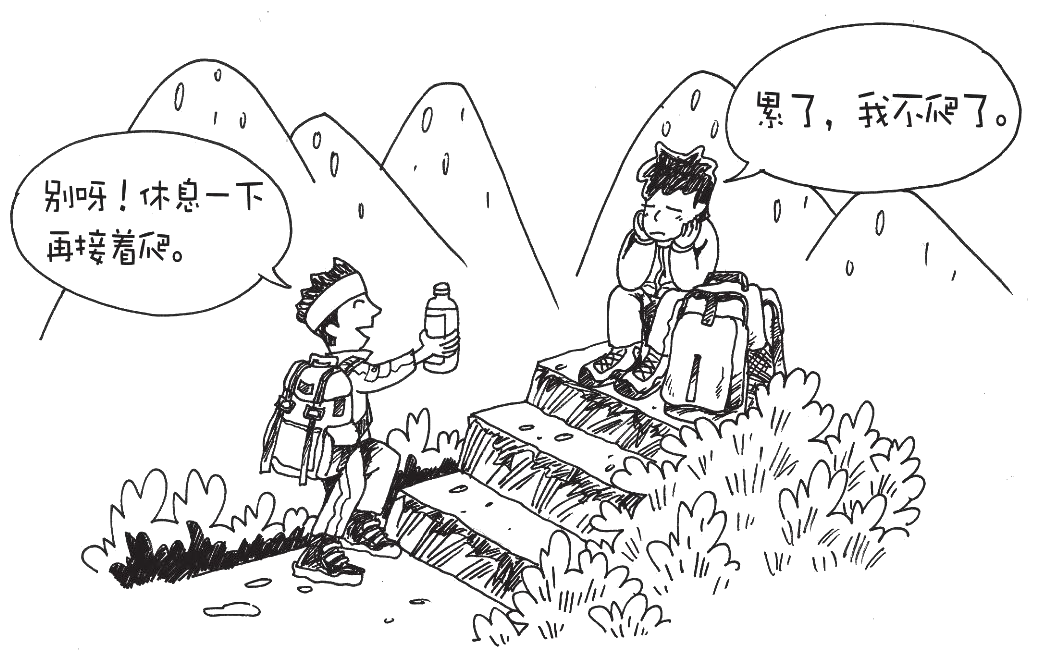
\includegraphics[width=0.58\linewidth]{picture/2019.png}
	\caption*{途中}
\end{figure}




